\clearpage
\twocolumn[{%
\rqparent
\subsection{Task reformulation}
\label{app:rq00_task_reformulation}

\noindent\begin{minipage}[t]{0.485\textwidth}
\vspace{0pt}
\paragraph{Research Question.} \emph{Do letter-format multiple-choice benchmarks leave chance at 90M--1.7B once the letters are dropped (\texttt{rf\_}) or the items are rewritten as cloze statements (\texttt{rfgm\_}), and do the reformulated twins then rank designs better?}

\paragraph{Setup.} We measure whether the letter-format benchmarks (Belebele, Global-MMLU, INCLUDE) pass the above-chance gate as published and after two reformulations of the same items. We call a reformulated task the twin of its original. RF drops the answer letters and scores each option as a continuation. LLM-RF has an LLM rewrite every item into a cloze statement with the options as its continuations (Belebele and INCLUDE only). We use the runs of the gate: seed 1904, every language setting, ladder and data build, 90M--1.7B, each task read on the runs that train its language. Each twin goes through the same gate as its original. A McNemar test on the paired verdicts of the original and its twin (one pair per task) tests the difference at every size.
\end{minipage}\hfill
\begin{minipage}[t]{0.485\textwidth}
\vspace{0pt}
\begin{rqfinding}
\textbf{1. Dropping the letters moves whole families across the gate.} At 1.7B the RF twins (\texttt{rf\_}) pass in 86 of 105 Belebele, 35 of 37 Global-MMLU and 31 of 43 INCLUDE tasks (tasks where only the twin passes against tasks where only the original passes: 82 : 1, 34 : 0 and 29 : 1, McNemar p $\leq$ 5.8e-08). (Figure~\ref{fig:app_rq00_task_reformulation}.)
\\
\\
\textbf{2. The margin gain is larger at 1.7B than at 90M.} The RF twins' median margin over chance exceeds the originals' by +0.030 / +0.017 / +0.004 at 90M and by \textbf{+0.098 / +0.058 / +0.047} at 1.7B (Belebele / Global-MMLU / INCLUDE).
\\
\\
\textbf{3. The Gemini rewrite gains more than dropping the letters.} At 1.7B the LLM-RF twins (\texttt{rfgm\_}) gain \textbf{+0.168} on Belebele (59 of 59 tasks significant) and \textbf{+0.075} on INCLUDE (21 of 36), against +0.098 and +0.047 for RF. \texttt{rfgm\_belebele} passes the gate in 59 of 59 tasks at every size, and \texttt{rfgm\_include\_base\_44} in 32 of 43 at 1.7B.
\end{rqfinding}
\end{minipage}

\vspace{\baselineskip}
\noindent\begin{minipage}{\textwidth}
\centering
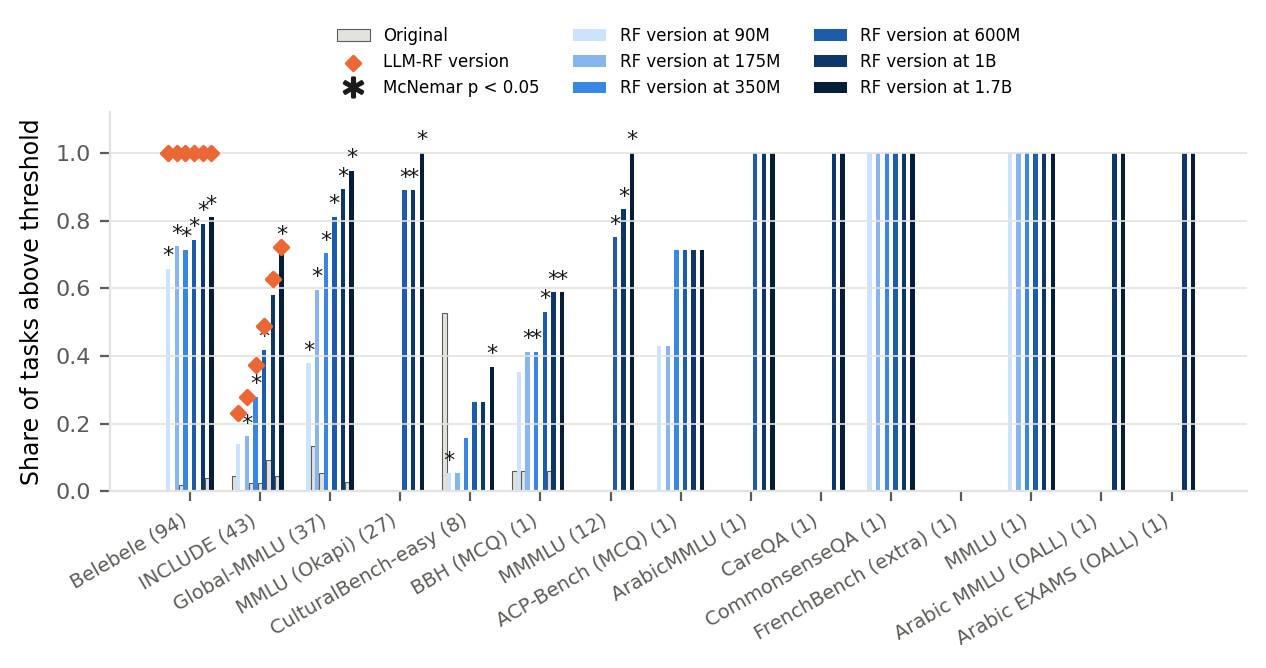
\includegraphics[width=\textwidth,height=0.36\textheight,keepaspectratio]{figures/app_rq00_chance_reformulation.png}
% source: src/signal-and-noise/analysis/rq00_task_reformulation/reformulations_gate_paper.png
\captionof{figure}{\textbf{Dropping the letters moves whole families across the gate.} For each letter-format benchmark (its number of tasks in parentheses), the share of tasks above the chance threshold for the original items (grey bars), for the RF version at each model size (blue bars, a darker blue is a larger size) and for the LLM-RF version (orange diamonds). A star marks a size at which the McNemar test between the original and its twin gives p $<$ 0.05.}
\label{fig:app_rq00_task_reformulation}
\end{minipage}
}]
